\section{Composantes de la mission}
\href{https://youtu.be/oWrt5QuPc0M}{Visualiser la Video}
\subsection{Objectif du processus d'ingénierie de mission spatiale}
L'objectif global du processus d'ingénierie de mission spatiale (présenté dans le chapitre précédent) est de définir un concept de mission de manière à inclure les composants suivants :
\begin{enumerate}
    \item Sujet  
    \item Charge utile  
    \item Bus spatial  
    \item Station au sol  
    \item Opérations de mission  
    \item Architecture de commande, de contrôle et de communication  
    \item Orbite  
    \item Segment de lancement  
\end{enumerate}
Ce cours se concentrera principalement sur la conception du bus spatial, mais abordera brièvement l'influence des autres composants sur sa conception.
\subsection{Sujet et Charge Utile}
La mission est centrée sur le sujet, qui comprend les phénomènes physiques ou les objets que le satellite doit observer, découvrir ou manipuler. Ces sujets peuvent inclure :
\begin{itemize}
    \item Les ondes gravitationnelles \textit{(GRACE)}
    \item Les fréquences d'Internet à large bande \textit{(Starlink)}
    \item Les astéroïdes \textit{(OSIRIS-REx)}
    \item Les neutrons \textit{(Neutron-1)}
\end{itemize}
Nous supposerons que vous avez abordé cette thématique en dehors de ce cours, par exemple dans \textit{EPET 301: Space Science Instrumentation}, ou avec vos collègues scientifiques et technologues qui sont vos clients. Vous pouvez également trouver des missions scientifiques ou technologiques intéressantes dans les enquêtes décennales de la NASA, ses plans stratégiques, ses feuilles de route et son rapport de taxonomie.

Le sujet influence les exigences orbitales si le satellite doit être proche de la source du sujet pour le détecter (comme pour \textit{OSIRIS-REx, GRACE} et \textit{Neutron-1}).
\subsection{Architecture de Commande, Contrôle et Communication}
\begin{itemize}
    \item L’architecture de commande, contrôle et communication est l’interface entre les opérations de mission, la station au sol et le satellite.
    \item Elle inclut le lien de télécommunication entre le satellite et la station au sol, ainsi que les connexions filaires ou sans fil entre la station au sol et le centre de contrôle de mission.
    \item Idéalement, le chemin du signal est aussi ininterrompu que possible pour permettre une transmission d’informations en temps réel, essentielle pour les missions à haute priorité.
    \item Pour les missions à faible priorité, les communications peuvent être retardées.
    \item Par exemple, il est possible de s’appuyer sur des opérateurs radioamateurs pour capter et transmettre les signaux, bien qu’il n’y ait aucune garantie qu’ils soient à l’écoute ou qu’ils transmettent les paquets reçus.
\end{itemize}

La charge utile est le matériel ou le logiciel qui détecte, mesure ou interagit avec le sujet. Si le sujet est le \textit{quoi}, la charge utile est le \textit{comment}. Il peut exister différents niveaux de charge utile si l'on élargit le périmètre du système. Par exemple :
\begin{itemize}
    \item Pour la mission \textit{Neutron-1}, la charge utile est un détecteur de neutrons.
    \item Si l'on considère la fusée qui lance \textit{Neutron-1} dans l'espace, la charge utile de la fusée est le satellite entier \textit{Neutron-1}.
\end{itemize}

Nous nous concentrerons strictement sur la charge utile intégrée au bus spatial, auquel une section entière sera dédiée, car le sujet et la charge utile influencent directement la conception du bus spatial.

\textbf{Kit Artemis CubeSat}
\begin{itemize}
    \item Une caméra opérant dans le spectre infrarouge et visible est incluse afin de favoriser les missions d'observation de la Terre et de la Lune.  
    \item Possibilité de retirer la caméra et d'utiliser un quart du volume du CubeSat pour une charge utile personnalisée.  
    \item Conception du bus spatial adaptable à une variété de :
    \begin{itemize}
        \item Connecteurs électriques  
        \item Tensions acceptables  
        \item Besoins en énergie  
    \end{itemize}
\end{itemize}
\subsection{Segment Sol}
Le segment sol comprend tous les composants restant au sol :  
\begin{itemize}  
    \item Station terrestre  
    \item Opérations de mission  
    \item Architecture de commande, de contrôle et de communication  
\end{itemize}
\begin{figure}[H] % H force l'affichage ici
    \centering
    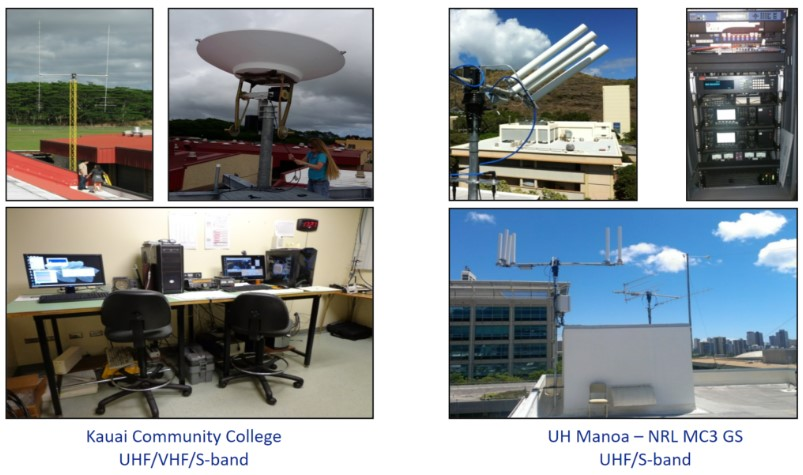
\includegraphics[width=0.8\textwidth]{figures/3.7.jpg}
    \caption{\href{https://www.hsfl.hawaii.edu/ground-stations/}{Examples of ground stations. Image Source: HSFL}}
    \label{fig:communication2}
\end{figure}
\textbf{Station Sol}

\begin{itemize}
    \item Une station sol est une \textit{« station radio terrestre con\^cue pour la t\'el\'ecommunication extraplan\'etaire avec un vaisseau spatial »}.
    \item R\^oles principaux :
    \begin{itemize}
        \item Communiquer et contr\^oler les engins spatiaux.  
        \item Recevoir des signaux faibles envoy\'es par le vaisseau spatial.  
        \item Transmettre des signaux puissants vers le vaisseau spatial.  
    \end{itemize}
    \item Caract\'eristiques des grandes stations sol :
    \begin{itemize}
        \item Antenne parabolique offrant une forte directivit\'e.  
        \item D\'etection de signaux radio sensibles provenant de sources astronomiques.  
        \item Exemples : \textbf{Deep Space Network} de la NASA.  
    \end{itemize}
    \item Les d\'ecouvertes astronomiques modernes utilisent des antennes plus grandes que celles n\'ecessaires aux communications spatiales.  
\end{itemize}
\begin{figure}[H] % H force l'affichage ici
    \centering
    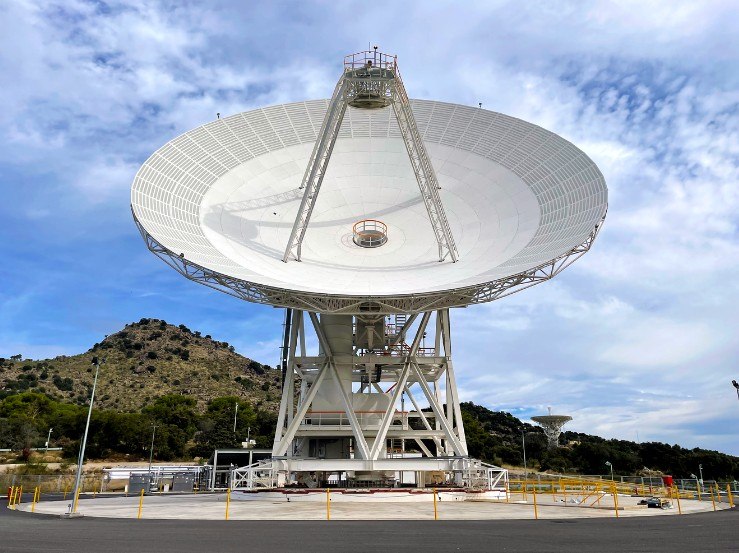
\includegraphics[width=0.8\textwidth]{figures/3.8-1.jpg}
    \caption{Example of a large dish in NASA’s Deep Space Network. Image courtesy of NASA.}
    \label{fig:communication2}
\end{figure}
\begin{figure}[H] % H force l'affichage ici
    \centering
    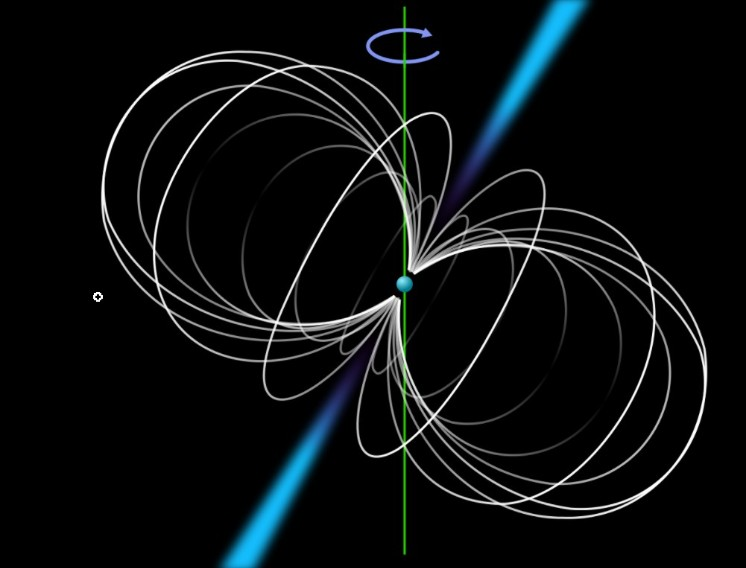
\includegraphics[width=0.8\textwidth]{figures/3.9.jpg}
    \caption{Example of an astronomical radio source. This is a schematic view of a pulsar. The sphere in the middle represents the neutron star, the curves indicate the magnetic field lines, the protruding cones represent the emission beams and the green line represents the axis on which the star rotates. Image by Roy Smits.}
    \label{fig:communication2}
\end{figure}
\textbf{Stations sol de petite taille}

\begin{itemize}
    \item Elles utilisent g\'en\'eralement un r\'eseau d'antennes dip\^oles, la classe d'antennes la plus courante dans la vie quotidienne.
    \item Caract\'eristiques :
    \begin{itemize}
        \item Omnidirectionnelles.  
        \item Construction simplifi\'ee.  
        \item Compr\'ehension th\'eorique plus accessible, ce qui les rend adapt\'ees aux \'equipes universitaires.  
    \end{itemize}
    \item Suivi des satellites :
    \begin{itemize}
        \item Les antennes, qu'elles soient de petite ou grande taille, peuvent \^etre fixes ou orientables pour suivre un satellite.
        \item Les grandes antennes directionnelles suivent rarement les signaux dynamiquement en raison de la complexit\'e des syst\`emes de support pour des masses importantes.
    \end{itemize}
    \item La construction des stations sol est hors du champ de ce cours, mais plusieurs options sont disponibles :
    \begin{itemize}
        \item Contacter \textbf{HSFL} pour un support missionnel.
        \item Planifier un acc\`es via les services \textbf{AWS Ground Station}.
        \item Participer \`a \textbf{SatNOGS}, un r\'eseau mondial open-source de stations sol.  
    \end{itemize}
\end{itemize}
\begin{figure}[H] % H force l'affichage ici
    \centering
    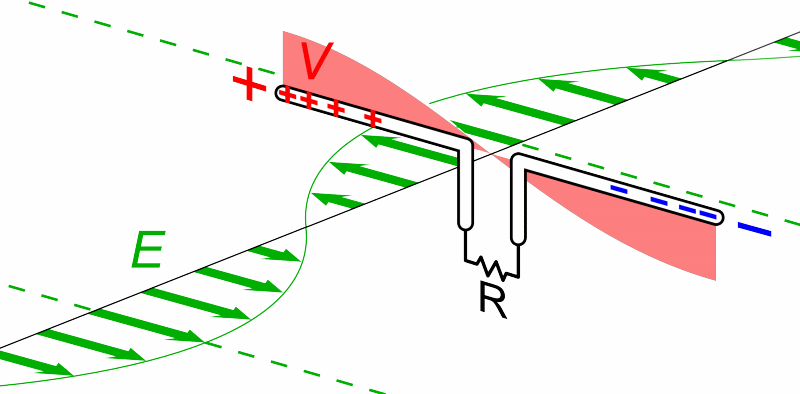
\includegraphics[width=0.8\textwidth]{Dipole_receiving_antenna_animation_6_800x394x150ms-2.png}
    \caption{Animated diagram of a half-wave dipole antenna receiving a radio wave. Image by Chet Vorno.}
    \label{fig:communication2}
\end{figure}

\subsection{Op\'erations de mission}
\begin{itemize}
    \item L'\'equipe des op\'erations de mission peut \^etre compos\'ee de sp\'ecialistes distincts dans un grand programme, comme les op\'erateurs du rover \textbf{Curiosity} de la NASA qui ont d\^u suivre une formation sp\'ecifique, ou bien des membres de l'\'equipe de conception du satellite pour les petits projets. 

    \item Si vous \^etes \'etudiant dans une petite \'equipe, vous serez tr\`es probablement l'un des op\'erateurs de mission ; et qui mieux que l'un des ing\'enieurs ayant con\c{c}u le satellite pour l'op\'erer ? Vous aurez l'avantage unique de conna\^itre pr\'ecis\'ement les capacit\'es du vaisseau spatial sans avoir besoin de consulter un ing\'enieur ext\'erieur, car cet ing\'enieur, c'est vous !  

    \item Le logiciel d'op\'erations de mission permet aux op\'erateurs de surveiller l'\'etat de sant\'e du vaisseau spatial ainsi que les param\`etres pertinents de la mission, tout en envoyant des commandes depuis un ordinateur. La NASA a d\'evelopp\'e \textbf{Open MCT}, un cadre de visualisation de donn\'ees de mission de nouvelle g\'en\'eration, bas\'e sur le Web, et con\c{c}u pour les environnements de bureau et mobiles.
\end{itemize}
\textbf{Sp\'ecificit\'es du kit Artemis}
\begin{itemize}
    \item Le kit Artemis CubeSat est fourni avec \textbf{COSMOS}, un package logiciel permettant le d\'eveloppement de logiciels de vol et offrant une interface pour les op\'erations de mission.
\end{itemize}
\begin{figure}[H] % H force l'affichage ici
    \centering
    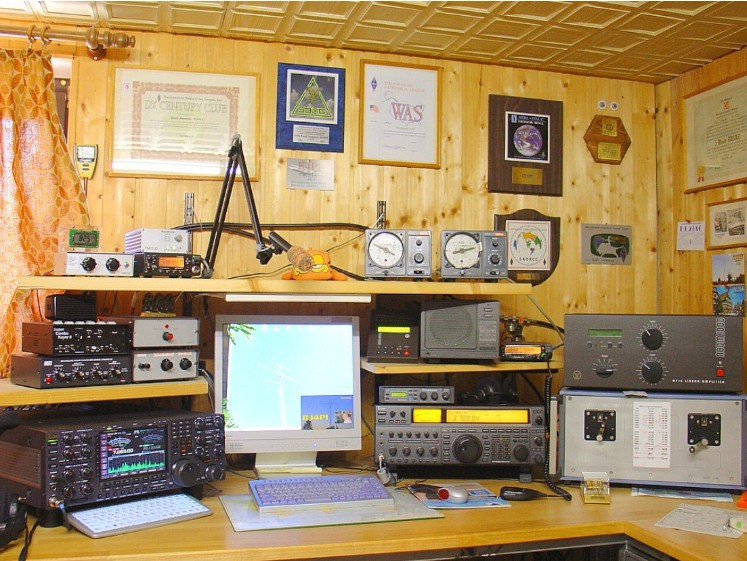
\includegraphics[width=0.8\textwidth]{figures/3.11.jpg}
    \caption{Example of amateur radio. Image by Emil Neuerer.}
    \label{fig:communication2}
\end{figure}
\textbf{Spécificité du Kit Artemis}
\begin{itemize}
    \item Pour le kit Artemis CubeSat, nous recommandons de collaborer avec HSFL.
    \item La conception du satellite intègre les stations au sol de HSFL, le logiciel d'opérations de mission et les interfaces correspondantes.
\end{itemize}

\textbf{Décision Critique sur l'Architecture de Communication}
\begin{itemize}
    \item Le choix de la \textbf{fréquence de communication} et l'obtention de la licence RF correspondante sont des étapes essentielles [CSLI Chapitre 9].
    \item Le kit \textbf{Artemis CubeSat} ne peut obtenir qu'une \textbf{licence radioamateur ou expérimentale}.
    \item Nous vous accompagnerons dans la documentation nécessaire pour l'obtention de la \textbf{licence FCC} [FCC Guidance et Spectrum Guidance].
    \item Ce processus est \textbf{complexe et soumis à des goulets d'étranglement}, mais des efforts sont en cours pour le simplifier.
    \item Les autorités gouvernementales travaillent à une simplification \textbf{du haut vers le bas}, tandis que nous cherchons à vous former \textbf{du bas vers le haut}.
\end{itemize}
\begin{figure}[H] % H force l'affichage ici
    \centering
    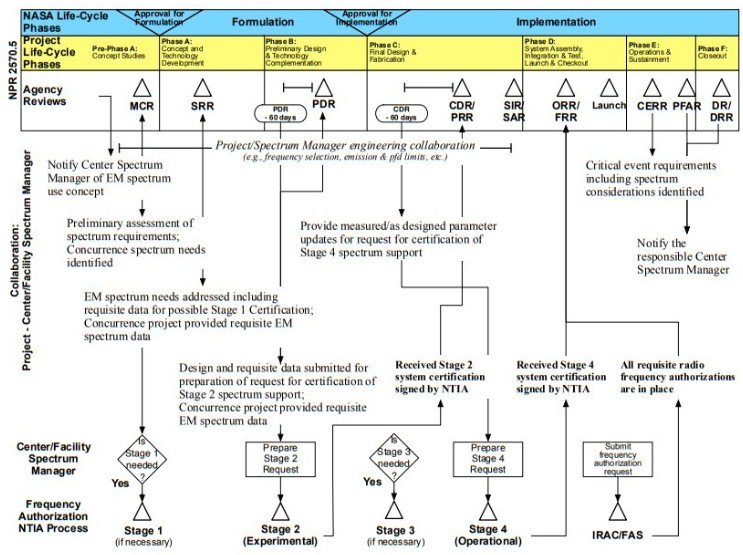
\includegraphics[width=0.8\textwidth]{figures/3.13.jpg}
    \caption{Spectrum certification process. Image courtesy of NASA.}
    \label{fig:communication2}
\end{figure}

\section*{Orbite et Lancement}

L'orbite correspond à la trajectoire du satellite au cours de sa mission par rapport aux corps planétaires et aux références astronomiques. Une section dédiée décrira en détail les différentes orbites et l’environnement spatial associé. Ce paragraphe offre une vue d’ensemble à un niveau plus global.

\begin{itemize}
    \item L’\textbf{orbite} détermine l’environnement spatial dans lequel le satellite doit évoluer ainsi que le lanceur avec lequel il doit être compatible.
    \item Les \textbf{caractéristiques orbitales} influencent les phénomènes physiques dominants dans cet environnement, imposant des exigences techniques spécifiques aux sous-systèmes du satellite pour atteindre l’objectif de la mission.
    \item L’\textbf{environnement spatial} peut également impacter les opérations de mission, en raison des délais de communication ou des interruptions de signal (\textit{blackouts}).
    \item La \textbf{distance} à parcourir ou le \textbf{delta-V} requis pour atteindre l’orbite souhaitée influence la taille du lanceur.
    \item Le lanceur impose des \textbf{contraintes de volume} en raison des dimensions de sa coiffe, dans laquelle le satellite doit s’intégrer.
\end{itemize}
\begin{figure}[H] % H force l'affichage ici
    \centering
    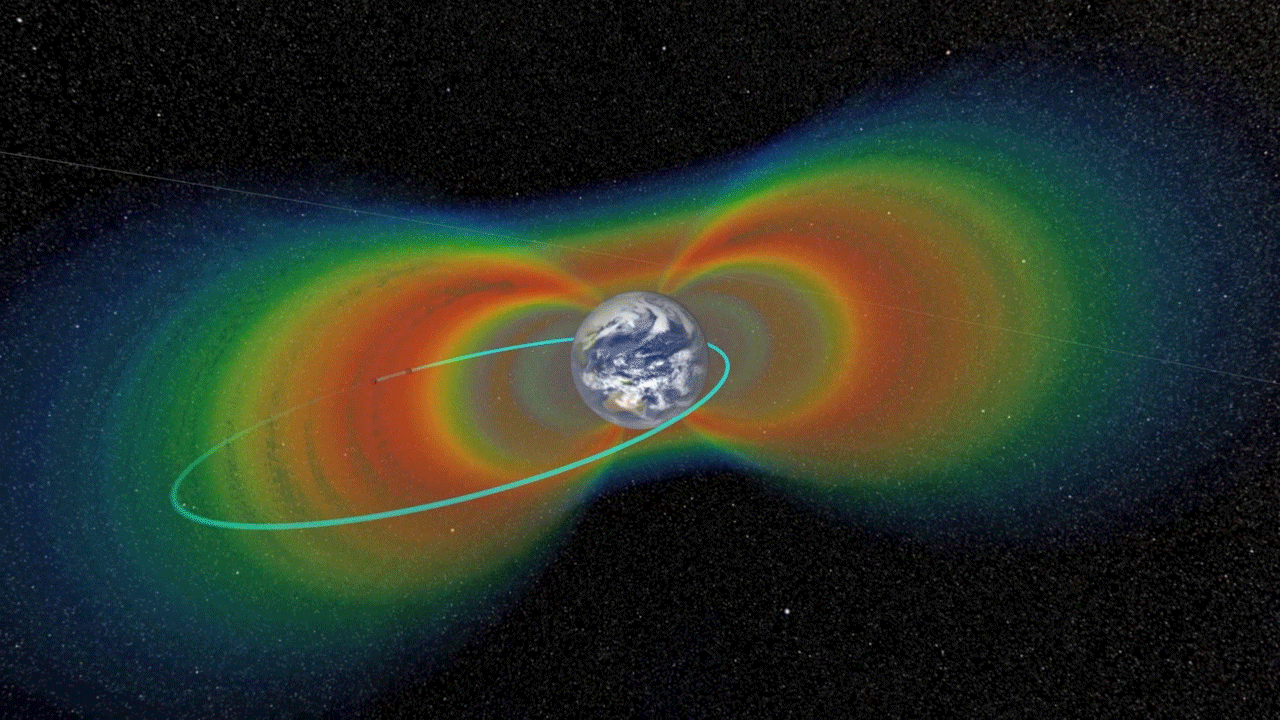
\includegraphics[width=0.8\textwidth]{figures/nasasvanalle.png}
    \caption{Example of an orbital path of a spacecraft. Image courtesy of Physics.org}
    \label{fig:communication2}
\end{figure}
\textbf{Spécificité du Kit Artemis}

\begin{itemize}
    \item Le matériel fourni avec le \textbf{kit Artemis CubeSat} est conçu pour fonctionner en \textbf{orbite basse terrestre} (LEO).
    \item Plus précisément, il est optimisé pour une \textbf{orbite similaire à celle de l’ISS}, car de nombreux CubeSats sont déployés depuis la Station Spatiale Internationale.
\end{itemize}
\textbf{Déploiement des CubeSats 1U}

\begin{itemize}
    \item Les \textbf{CubeSats 1U} sont généralement \textbf{intégrés dans des déployeurs} au sol.
    \item Ils sont ensuite \textbf{transportés vers l’ISS} dans un \textbf{vaisseau cargo pressurisé} (par exemple, \textbf{SpaceX Dragon} ou \textbf{Orbital ATK Cygnus}).
    \item Une fois à bord de l’ISS, ils sont \textbf{manipulés manuellement} par les astronautes.
    \item Les CubeSats sont habituellement \textbf{déployés de l’ISS 1 à 3 mois après leur arrivée} [CSLI Chapitre 3.5].
\end{itemize}

\textbf{Spécificités du Kit Artemis}
\begin{itemize}
    \item Si le \textbf{CubeSat Artemis} n’est pas stocké en douceur (\textit{softly stowed}), 
    \item Le kit a été testé selon les \textbf{normes NASA CSLI} pour survivre au \textbf{ridesharing} en tant que \textbf{charge utile auxiliaire} montée directement sur les lanceurs [NASA GEVS].
\end{itemize}

\begin{itemize}
    \item Si vous choisissez de lancer en dehors de l'écosystème \textbf{CSLI}, comme \textbf{UNP},  
    \item Vous pouvez trouver d'autres \textbf{fournisseurs de lancement} avec leurs propres normes de tests environnementaux.
    \item Idéalement, ces normes sont \textbf{moins rigoureuses} que celles du \textbf{CSLI}, 
    \item Ce qui éviterait de refaire tous les tests environnementaux que nous avons déjà réalisés pour vous.
\end{itemize}
\begin{figure}[H] % H force l'affichage ici
    \centering
    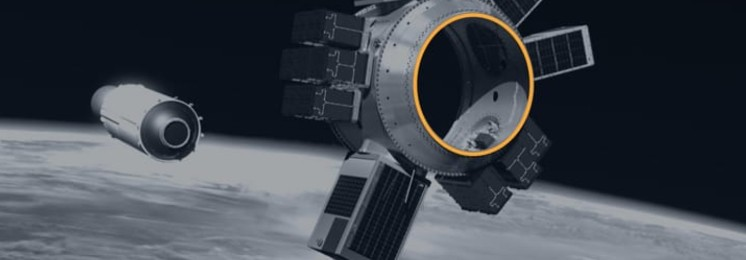
\includegraphics[width=0.8\textwidth]{3.14.jpg}
    \caption\href{https://blog.satsearch.co/2019-12-04-find-a-launch-option-for-your-cubesat-or-small-satellite-an-overview-of-launch-service-providers}{Select a launch provider for your CubeSat. Image courtesy of Spaceflight Industries.}
    \label{fig:communication2}
\end{figure}
\subsection{Bus Spatial}
\begin{itemize}
    \item Lors de la conception préliminaire, il est recommandé d'allouer des budgets de \textbf{masse} et de \textbf{puissance} pour un satellite sans propulsion.
    \item Un \textbf{ingénieur systèmes} est généralement chargé du suivi de ces budgets, ainsi que d'autres paramètres tels que :
    \begin{itemize}
        \item L'alignement et le pointage pour l'\textbf{ADCS}.
        \item Le \textbf{propulseur}, si le satellite est propulsif.
        \item La \textbf{liaison montante et descendante} pour les communications.
        \item L'utilisation des données pour le \textbf{traitement des commandes et des données}.
    \end{itemize}
    \item Ces budgets seront détaillés dans les sections consacrées aux sous-systèmes correspondants.
\end{itemize}

\begin{table}[h]
    \centering
    \begin{tabular}{|l|c|c|c|}
        \hline
        \textbf{Sous-système} & \textbf{SMAD sugg} & \textbf{Hermes CubeSat} & \textbf{Artemis CubeSat} \\
        \hline
        Charge utile & 41\% & Allocated in T\&C & 2\% \\
        \hline
        Structure et Mécanismes & 20\% & 32.3\% & 20\% \\
        \hline
        Contrôle thermique & 2\% & 0\% & 0\% \\
        \hline
        Puissance (y compris harnais) & 19\% & 13.5\% & 48\% \\
        \hline
        Télémétrie et Contrôle & 2\% & 22.5\% & 5\% \\
        \hline
        Commande et Traitement des Données & 5\% & 3.6\% & 18\% \\
        \hline
        Détermination et Contrôle d'Attitude & 8\% & 2.4\% & 8\% \\
        \hline
        Autres (équilibrage + lancement) & 3\% & 25.7\% & 0\% \\
        \hline
        \textbf{Total} & 100\% & 100\% & 100\% \\
        \hline
    \end{tabular}
    \caption{Répartition de la masse sèche des sous-systèmes des CubeSats}
    \label{tab:subsystem_mass}
\end{table}




